\chapter{Concepts et méthodes de base}
\label{chap:concepts}

Ce chapitre présente les concepts qui sont importants pour comprendre le contexte dans lequel s'inscrit cette thèse.
Nous décrivons tout d'abord l'indexation de documents scientifiques, qu'elle soit manuelle ou automatique.
Nous nous intéressons ensuite aux mots-clés et à leurs principales caractéristiques.
Enfin, nous présentons un état de l'art des méthodes d'extraction de mots-clés en chaîne de traitement, en commençant par décrire les trois étapes de cette chaîne: l'identification de candidats, leur pondération, puis la sélection d'un ensemble de mots-clés parmi ces candidats. Nous présenterons dans le chapitre suivant un état de l'art des méthodes neuronales de bout-en-bout.



\section{Indexation de documents scientifiques}


L'indexation est un processus qui vise à identifier les éléments notables d'un document dans le but de le caractériser~\cite{khemiri_manual_2020}.
L'indexation par mots-clés, ou association de mots-clés à des documents, est à l'origine un processus manuel, effectué par des indexeurs professionnels ou des bibliothécaires formés à cette problématique.
Dans les bibliothèques, les documents sont généralement associés à des mots-clés qui proviennent de vocabulaires contrôlés.
Par exemple, les bibliothèques universitaires indexent leurs documents grâce au langage documentaire RAMEAU~\cite{centre_national_rameau_guide_2017} qui permet de décrire les sujets des documents grâce à des descripteurs.
Dans ce langage documentaire, un document intitulé \say{Les événements de mai 68 racontés par un étudiant} sera indexé avec les descripteurs suivants: France -- 1968 (Journées de mai) -- Récits personnels; ou encore le document \say{Les conditions de travail des enseignants en Bretagne} sera indexé de la manière suivante: Enseignants -- France -- Bretagne (France) -- Conditions de travail.\footnote{Exemples extraits de \url{https://rameau.bnf.fr/sites/default/files/formation/pdf/ex2corr.pdf}}

\subsection{Indexation manuelle}
\label{sub:concepts_indexation_manuelle}

L'indexation manuelle par mots-clés, appelée aussi annotation manuelle de documents en mots-clés, peut s'effectuer de manière contrôlée ou non contrôlée.
De manière contrôlée, les mots-clés sont à choisir dans un référentiel (ontologie, thésaurus, base de données terminologiques, etc.). De manière non contrôlée, le choix des mots-clés est à la discrétion de l'annotateur.
Pour illustrer cette indexation par mots-clés, nous présentons dans la figure~\ref{fig:ex_termith} un exemple de notice scientifique annotée en mots-clés par des indexeurs professionnels.

\begin{figure}
    \centering
    %\centerfloat
    \resizebox{0.98\textwidth}{!}{%
    \begin{tabular}{|p{1.3\textwidth}|}
    \textbf{\textcolor{color3}{Agrégats} de \textcolor{color8}{mots-clés} validés sémantiquement: Pour de nouveaux services d'accès à l'information sur internet} (id: \texttt{ sciencesInfo\_10-0065090\_tei})  
    \vspace{0.5em}


    A l'heure du web \textcolor{color2}{social}, nous présentons une solution destinée à définir de nouveaux services tels que \textcolor{color1}{la} construction automatique et dynamique de \textcolor{color1}{communautés} d'utilisateurs: l'agrégation de \textcolor{color8}{mots-clés}. Ces \textcolor{color3}{agrégats} de \textcolor{color8}{mots-clés} sont issus des \textcolor{color6}{recherches} antérieures des utilisateurs réalisées au travers d'un moteur de \textcolor{color6}{recherche}. Nous présentons la démarche que nous avons suivie pour obtenir un \textcolor{color0}{algorithme} de regroupement des \textcolor{color8}{mots-clés} provenant de \textcolor{color4}{fichiers} de traçage (\textcolor{color5}{log}) ; nous illustrons cet \textcolor{color0}{algorithme} au travers de son application au \textcolor{color4}{fichier} de traçage du moteur de \textcolor{color6}{recherche} aol.com. A des fins d'évaluation et de validation, nous proposons de comparer les résultats obtenus par le moteur de \textcolor{color6}{recherche} à partir des \textcolor{color3}{agrégats} de \textcolor{color8}{mots-clés} ainsi créés et de définir un coefficient de cohérence sémantique de ces \textcolor{color3}{agrégats}. Nous mesurons dans une expérimentation la perte de cohérence sémantique liée à l'augmentation de la taille des \textcolor{color3}{agrégats}. L'intérêt de notre approche réside dans le fait qu'elle peut être considérée comme une brique de base pour un grand nombre de systèmes « communautaires » et ainsi exploitée pour offrir encore plus de services à l'usager.    
    \vspace{0.5em}
    
    \textbf{Mots-clés de référence:} Classe, \textcolor{color4}{Fichier}~\textcolor{color5}{log}, \textcolor{color3}{Agrégat}, \textcolor{color8}{Mot~clé}, Traitement~de~la~requête, \textcolor{color1}{Communauté}~virtuelle, Réseau~\textcolor{color2}{social}, \textcolor{color6}{Recherche}~information, \textcolor{color0}{Algorithme}
    \end{tabular}%
    }
    \caption{Exemple de notice scientifique des bases bibliographiques Pascal et Francis. Les mots communs entre le document et les mots-clés sont colorés.}
    \label{fig:ex_termith}
\end{figure}

L'annotation contrôlée permet d'assurer une cohérence dans le choix des termes mais limite le nombre de concepts. Elle nécessite aussi une connaissance experte du référentiel utilisé, par exemple le MeSH dans le domaine médical, c'est pourquoi des indexeurs professionnels sont formés à leur utilisation. Le MeSH contient \num{25 186} termes\footnote{\url{https://www.nlm.nih.gov/databases/download/mesh.html}} organisés hiérarchiquement avec quatre niveaux de profondeur en moyenne.
%
%Pour l'annotation des documents des consignes sont généralement fournies par les bibliothèques. Par exemple, la National Library of Medicine\footnote{\url{https://www.nlm.nih.gov/bsd/indexing/training/TIP_010.html}} qui gère PubMed recommande d'identifier les mots-clés des documents en ne prenant en compte que certaines parties des documents~: le résumé, l'introduction, les résultats, la conclusion et les mots mis en emphase.
%
Pour faciliter cette annotation contrôlée, des outils d'annotation semi-automatique, tels que le Medical Text Indexer~\cite{mork_nlm_2013} pour PubMed, suggèrent aux indexeurs les mots-clés du référentiel qui apparaissent dans les documents.
Les indexeurs procèdent ensuite à un examen manuel des mots-clés suggérés pour valider ou ajouter des mots-clés du référentiel qui n'ont pas été détectés par ces outils.
%
En contrepartie de la qualité de ces référentiels, leur mise à jour et leur construction sont de lourds processus qui doivent toujours prendre en compte l'intégralité du référentiel pour garantir sa cohérence. %Le maintien des référentiels nécessite l'ajout et la suppression permanente de nouveaux termes, la modification des termes préférés en fonction des usages, etc.

L'indexation non contrôlée, contrairement à l'indexation contrôlée, n'est soumise à aucune contrainte. Elle permet une annotation réalisable sans connaissances préalables mais impacte négativement la cohérence de l'annotation d'un document à l'autre. Cette incohérence est montrée dans la figure~\ref{tab:variants} qui regroupe les variantes du concept de \foreign{neural network} dans des documents scientifiques annotés par leurs auteurs.
L'indexation non contrôlée permet aussi, contrairement à l'indexation contrôlée, d'indexer des concepts émergeant et n'est pas limitée aux termes déjà identifiés par un référentiel.
Cette indexation non contrôlée est principalement utilisée dans les bibliothèques numériques scientifiques, car les documents qui comportent des mots-clés sont pour la plupart annotés par leurs auteurs lors de l'écriture ou de la soumission des articles.

\iffalse
\begin{table}[htb!]
    \centering
    \begin{tabular}{lr}
        \toprule
        \textbf{Variantes racinisées} & \textbf{Fréquence} \\
        \midrule
        neural network & 5612 \\
        artifici neural network & 2083 \\
        artifici neural network (ann)  & 147 \\
        neural net  & 138 \\
        neural network model & 79 \\
        neural model  & 70 \\
        neural network (nn)  & 36 \\
        artifici neural network (anns) & 34 \\
        ann artifici neural network & 25 \\
        neural network (nns) & 24 \\
        neural-network & 9 \\
        the neural network & 8 \\
        artifici neural network model & 7 \\
        neural network (computer) & 7 \\
        nn & 7 \\
        artifici neural net & 6 \\
        nn neural network & 6 \\
        artif neural network & 4 \\
        neural networks. & 3 \\
        ann (artifici neural net) & 2 \\
        ann (artifici neural networks) & 2 \\
        artifici neural network (anni)  & 1 \\
        ann: artifici neural network  & 1 \\
        arti?ci neural network & 1 \\
        artifici neural networks. cad & 1 \\
        ann ann artifici neural network & 1 \\
        nn nn neural network & 1 \\
        \bottomrule
    \end{tabular}
    \caption{Variantes du concept de \textit{neural network} trouvées dans les mots-clés de référence de KP20k.}
    %\label{tab:variants}
\end{table}
\fi

\begin{figure}[htb!]
    \centering
    \resizebox{0.9\textwidth}{!}{
    \begin{tabular}{lr|lr}
        \toprule
        \textbf{Variantes racinisées} & \textbf{Fréquence} & \textbf{Variantes racinisées (\textit{suite})} & \textbf{Fréquence} \\
        \midrule
neural network & 5612 & nn & 7 \\
artifici neural network & 2083 & artifici neural net & 6 \\
artifici neural network (ann)  & 147 & nn neural network & 6 \\
neural net  & 138 & artif neural network & 4 \\
neural network model & 79 & neural networks. & 3 \\
neural model  & 70 & ann (artifici neural net) & 2 \\
neural network (nn)  & 36 & ann (artifici neural networks) & 2 \\
artifici neural network (anns) & 34 & artifici neural network (anni)  & 1 \\
ann artifici neural network & 25 & ann: artifici neural network  & 1 \\
neural network (nns) & 24 & arti?ci neural network & 1 \\
neural-network & 9 & artifici neural networks. cad & 1 \\
the neural network & 8 & ann ann artifici neural network & 1 \\
artifici neural network model & 7 & nn nn neural network & 1 \\
        \bottomrule
    \end{tabular}
    }
    \caption{Variantes racinisées du concept de \textit{neural network} trouvées dans les mots-clés de référence de KP20k.}
    \label{tab:variants}
\end{figure}



L'annotation en mots-clés, qu'elle soit contrôlée ou non, est généralement effectuée par des auteurs, des lecteurs ou des indexeurs professionnels.\\
Les \textbf{auteurs} fournissent des mots-clés pour les documents qu'ils ont écrits, ils ont donc une connaissance experte du domaine et du contenu du document.
Les mots-clés qu'ils choisissent décrivent les concepts importants de leur point de vue et peuvent omettre certains concepts abordés.
De plus, le choix des mots-clés peut être biaisé par les thématiques populaires du moment dans le but d'augmenter la visibilité de l'article.
L'annotation par les auteurs est très peu cohérente car il n'y a pas de guide d'annotation, et chaque document est annoté par une personne différente.
La figure~\ref{tab:variants} présente des variantes du concept de \foreign{neural network} (\say{réseau de neurone} en français) annotés par des auteurs.\\
Les \textbf{lecteurs}, quant à eux, ne sont pas des experts de l'annotation mais peuvent être experts du domaine du document. Au contraire des auteurs, leur but n'est pas la visibilité du document mais plutôt l'identification des concepts des documents qui leur sont personnellement utiles dans leur recherche documentaire.
Les annotations lecteurs -- dans le cadre de documents scientifiques -- proviennent généralement de plateformes de partage de bibliographies dans lesquels les utilisateurs peuvent associer des mots-clés à des documents.
Dans un cadre de création de jeux de données pour la production automatique de mots-clés, les données des utilisateurs sont compilées et filtrées pour obtenir un ensemble de mots-clés associé à chaque document retenu.
% Les annotations lecteurs peuvent être constituée en exploitant la folksonomie, c'est-à-dire une annotation des documents par plusieurs lecteurs suivie de règles pour ne conserver qu'une partie de ces mots-clés (souvent les plus assignés).
%Ce type d'annotation est mis en place sur des sites de partage de signets, dans lesquels les utilisateurs assignent des mots-clés à des ressources internets qui sont ensuite partagé aux autres utilisateurs.
%L'annotation en mots-clés par des lecteurs s'effectue majoritairement dans le cadre de création de jeux de données.
Cette annotation lecteur permet, par exemple, d'offrir une annotation alternative à une annotation déjà présente ou tout simplement d'obtenir une annotation en mots-clés moins coûteuse qu'une annotation professionnelle.\\
Les \textbf{indexeurs professionnels}, pour leur part, sont formés à l'indexation et à l'utilisation de langages documentaires.
Ils peuvent avoir une expertise dans le domaine des documents à annoter et ont pour objectif d'affecter des mots-clés qui facilitent la recherche documentaire pour les utilisateurs.
%L'annotation des jeux de données par des lecteurs s'effectue selon des protocoles très différents allants d'une simple annotation humaine sans vérification à des protocoles exigeants en termes de qualité. Il est facile d'imaginer que dans le premier cas, les extractions seront privilégiées.


Pour illustrer la différence d'annotation entre les auteurs et les indexeurs professionnels, nous comparons le nombre de mots-clés assigné aux documents par ces deux types d'annotateurs. Ainsi, la figure~\ref{fig:kw_per_doc_abstract} présente la fréquence de documents par nombre de mots-clés pour trois jeux de données de notices scientifiques: Inspec et KP20k en anglais; TermITH-Eval en français.
La différence entre l'annotation indexeur et l'annotation auteur est flagrante. En effet, les auteurs assignent le plus souvent cinq mots-clés par document, ce qui correspond au nombre maximal de mots-clés autorisés par les éditeurs de documents scientifiques, alors que les indexeurs, qui ne sont pas contraints par un seuil maximal, annotent en majorité de 6 à 10 mots-clés par document, sans différence entre le français et l'anglais.
\begin{figure}
    \centering

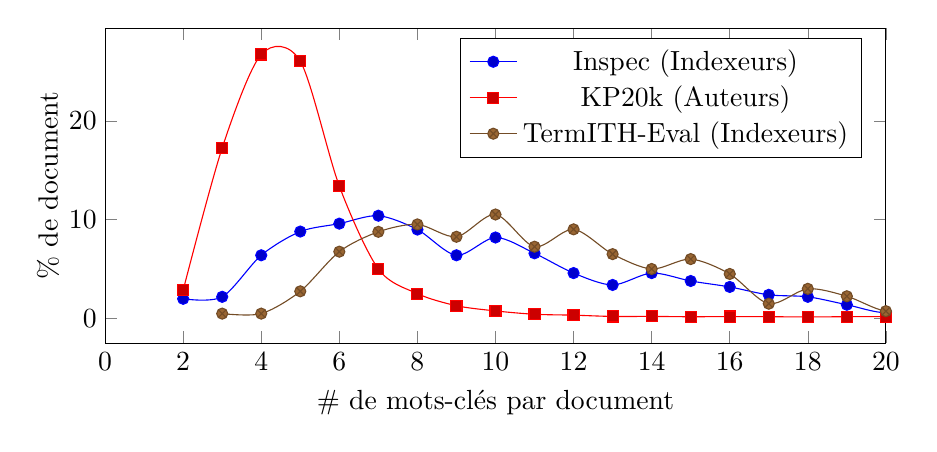
\begin{tikzpicture}
\begin{axis}[
    scale only axis,
    width=\textwidth-0.1cm-60,
    height=4cm,
    yticklabel style={inner sep=0pt, align=right, xshift=-0.1cm},
    xmin=0, xmax=20,
    xlabel={\# de mots-clés par document},
    ylabel={\% de document},
    %legend columns=2,
    legend pos=north east]

%\addlegendentry{KDD}
%\addplot+[smooth] coordinates {
%    (1, 6.22516556)(2, 8.74172185)(3, 22.38410596)(4, 28.21192053)(5, 14.56953642)(6, 12.31788079)(7, 4.10596026)(8, 2.1192053)(9, 0.39735099)(10, 0.66225166)(12, 0.13245033)(13, 0.13245033)};

\addlegendentry{Inspec (Indexeurs)}
\addplot+[smooth] coordinates {
    (2, 2.)(3, 2.2)(4, 6.4)(5, 8.8)(6, 9.6)(7, 10.4)(8, 9.)(9, 6.4)(10, 8.2)(11, 6.6)(12, 4.6)(13, 3.4)(14, 4.6)(15, 3.8)(16, 3.2)(17, 2.4)(18, 2.2)(19, 1.4)(20, 0.6)(21, 1.6)(22, 0.8)(23, 0.8)(24, 0.2)(26, 0.2)(27, 0.2)(28, 0.2)(31, 0.2)};
    
\addlegendentry{KP20k (Auteurs)}
\addplot+[smooth] coordinates {
    (2, 2.865)(3, 17.26)(4, 26.705)(5, 26.02)(6, 13.395)(7, 5.01)(8, 2.52)(9, 1.3)(10, 0.775)(11, 0.435)(12, 0.345)(13, 0.215)(14, 0.22)(15, 0.185)(16, 0.205)(17, 0.19)(18, 0.165)(19, 0.19)(20, 0.195)(21, 0.23)(22, 0.12)(23, 0.165)(24, 0.125)(25, 0.09)(26, 0.115)(27, 0.085)(28, 0.125)(29, 0.085)(30, 0.1)(31, 0.085)(32, 0.075)(33, 0.055)(34, 0.055)(35, 0.055)(36, 0.045)(37, 0.01)(38, 0.015)(39, 0.01)(40, 0.025)(41, 0.005)(42, 0.02)(43, 0.01)(44, 0.01)(45, 0.005)(46, 0.005)(47, 0.015)(51, 0.005)(52, 0.005)(54, 0.005)(55, 0.005)(57, 0.005)(59, 0.005)(60, 0.005)(65, 0.005)(68, 0.01)(77, 0.005)(97, 0.005)(100, 0.005)};

\addlegendentry{TermITH-Eval (Indexeurs)}
\addplot+[smooth] coordinates {
    (3, 0.50125313)(4, 0.50125313)(5, 2.75689223)(6, 6.76691729)(7, 8.77192982)(8, 9.52380952)(9, 8.27067669)(10, 10.52631579)(11, 7.26817043)(12, 9.02255639)(13, 6.51629073)(14, 5.01253133)(15, 6.01503759)(16, 4.5112782)(17, 1.5037594)(18, 3.0075188)(19, 2.2556391)(20, 0.7518797)(21, 1.25313283)(22, 1.00250627)(23, 0.50125313)(24, 1.25313283)(25, 0.7518797)(26, 0.25062657)(28, 0.25062657)(30, 0.25062657)(31, 0.50125313)(33, 0.25062657)(37, 0.25062657)};

\end{axis}
\end{tikzpicture}


    \caption{Nombre de mots-clés par document annoté par différentes catégories d'annotateurs.}
    \label{fig:kw_per_doc_abstract}
\end{figure}


%intro du chapitre
\subsection{Indexation automatique par mots-clés}

%1. c'est quoi l'indexation automatique
% pourquoi ça c'est imposé: plus de doc, cout d'indexation manuelle, temps de traitement
%3. il y a de l'indexation automatique plein texte qui utilise tout les mots du doc comme termes d'indexe
%4. pour compléter/améliorer l'index auto et faciliter l'indexation manuelle on fait de l'AKE, faire de la recherche à facette, créer des vocabulaire contrôlé pour ensuite annoter les documents, faire des résumé à utiliser au lieu de texte plein ?
% Donc les mots-clés blablabla

L'indexation automatique consiste à caractériser des documents de manière automatique, c'est-à-dire à choisir et à pondérer les descripteurs d'un document de manière automatique.
L'indexation plein texte est un type d'indexation automatique qui considère chaque mot du document comme un descripteur potentiel, puis lui attribue un poids selon un schéma de pondération tel que \tfidf{}.

Les techniques d'indexation automatique ont été développées pour simplifier et accélérer le travail d'indexation jusque-là manuel. Ce travail nécessite la disponibilité d'experts ainsi que des budgets conséquents: l'annotation manuelle d'un article de PubMed coûte une dizaine de dollars\footnote{\href{https://lhncbc.nlm.nih.gov/ii/information/about.html}{lhncbc.nlm.nih.gov/ii/information/about.html}}; en 2020, 1,5 million d'articles ont été ajoutés à PubMed ce qui représente un budget de 10,5 millions de dollars pour cette seule année.
Ce processus est aussi coûteux en temps: il faut compter entre 2 et 3 mois entre la soumission d'un document et son indexation. Ce délai d'attente découle de la masse de documents à indexer. 

%Par rapport à une indexation manuelle qui permet le prise en compte de variantes telles que les synonymes, l'indexation plein texte elle ne comprend que les mots apparaissant dans le document.

Nous nous intéressons ici à l'indexation automatique par mots-clés que nous considérons comme un type d'indexation libre. Et plus particulièrement, nous nous intéressons à la production automatique de mots-clés.
Les mots-clés sont des unités textuelles qui représentent les sujets importants d'un document. Nous les présenterons en détail dans la section~\ref{sec:caracterisation_keywords}.
Les mots-clés ont de multiples intérêts pour l'indexation automatique de documents: ils peuvent aider à la création de thésaurus~\cite{kosovac_use_2002} ou autre référentiel; ils peuvent aussi aider à la création de résumés automatiques~\cite{litvak_graph-based_2008,qazvinian_citation_2010}. Par ailleurs, ils peuvent enrichir l'indexation plein texte ou encore être utilisés pour de la recherche à facette~\cite{gutwin_improving_1999}. % intérêt direct, indirect

La tâche qui consiste à associer automatiquement des mots-clés à des documents est généralement nommée \say{extraction de mots-clés} (\foreign{keyphrase extraction}) \cite{hasan_automatic_2014, meng_deep_2017}.
La grande majorité des méthodes de production automatique de mots-clés proposée avant 2017 sont extractives, c'est-à-dire qu'elles produisent des mots-clés présents dans le document.
En 2017, \citet{meng_deep_2017} introduit une méthode supervisée générative qui génère des mots-clés mot-à-mot à partir d'un vocabulaire. Cette méthode permet donc non seulement de produire des mots-clés présents mais aussi des mots-clés absents du document.
%Les mots-clés absents qui jusque là attiraient peu d'attention car difficile à produire connaissent maintenant un intérêt grandissant.

Le terme \say{extraction de mots-clés} est ambigu: il peut désigner la seule production de mots-clés présents, ou bien la production de mots-clés indifféremment présents ou absents. Dans ce travail de thèse, nous réservons le terme d'extraction de mots-clés à la seule extraction de mots-clés apparaissant dans le document. Pour l'affectation de mots-clés à un document, qu'ils soient présents ou absents du document, nous emploierons \say{assignation de mots-clés} si les mots-clés proviennent d'un vocabulaire contrôlé et \say{génération de mots-clés} si les mots-clés sont générés par des modèles supervisés ou semi-supervisés. 
Le terme \say{production de mots-clés} désignera indifféremment l'extraction, l'assignation ou la génération de mots-clés.

%Les mots-clés ne sont en pratique que peu utilisé pour l'indexation automatique. D'une part car ils sont peu disponible, et comme nous l'avons vu, nécessitent soit des indexeurs professionnels soit la mise en \oe{}vre d'outils automatique de production de mots-clés.
%Notons leur utilisation dans les bibliothèques en accès libre ISTEX pour l'indexation et dans Microsoft Academics et ArnetMiner comme facettes.

\section{Définition et caractéristiques des mots-clés} \label{sec:caracterisation_keywords}

Dans cette section nous examinons deux propriétés des mots-clés: les catégories grammaticales de leurs composants et leur longueur. Nous illustrons ces propriétés à l'aide de deux jeux de données: KP20k pour l'anglais et TermITH-Eval pour le français.

Dans la littérature, \say{mots-clés} et \say{termes-clés} sont utilisés de manière interchangeable pour désigner les concepts importants d'un document.
\footnote{\say{descripteurs} peut aussi être utilisé dans le contexte de la recherche d'informations.}
% aussi descripteurs
Ces deux appellations peuvent parfois être utilisées afin de différencier les mots-clés comprenant plusieurs mots (termes-clés) des unigrammes (mots-clés) mais cette utilisation n'est pas systématique.
Dans ce travail de thèse, nous choisissons d'employer \say{mot-clé} pour désigner ces concepts importants sans rapport avec le nombre de mots qui les composent, ni le fait que les \say{mots-clés} soient des termes (d'un point de vue terminologique).\footnote{Les travaux de \cite{bougouin_indexation_2015} portent sur les domaines de spécialité d'où son utilisation de \say{terme-clé}.}

L'indexation des documents se fait toujours en leur associant des ensembles de mots-clés. Ces ensembles doivent respecter les propriétés de non-redondance et de couverture, c'est-à-dire que les mots-clés qui les composent doivent être sémantiquement disjoints, et couvrir le plus de concepts importants du document~\cite{firoozeh_keyword_2020}.
Au niveau d'une collection de documents, les mots-clés peuvent être plus ou moins cohérents, c'est-à-dire qu'un concept est représenté par un nombre plus ou moins grand de variantes. L'exemple du concept de \foreign{neural network} dans la figure~\ref{tab:variants} met en lumière ce phénomène.
% \cite{harpring_introduction_2010} à propos des controlled lists: In a well-constructed controlled list, the following is true: each term is unique; terms are not overlapping in meaning; terms are all members of the same class (i.e., having the same level of rank in a classifica tion system); terms are equal in granularity or specificity; and terms are arranged alphabetically or in another logical order

\subsection{Nature linguistique des mots-clés}
\label{sub:nature_linguistique}

Dans cette section, nous définissons les caractéristiques linguistiques des mots-clés.
Selon l'étude de \citet{hulth_improved_2003} les mots-clés sont majoritairement des noms et des expressions nominales, et sont donc composés de noms et d'adjectifs.
% présente les 5 patrons morphosyntaxiques les plus fréquents dans le jeu de données anglais Inspec sont du plus au mois fréquent:  \texttt{ADJ~NOUN}; \texttt{NOUN~NOUN}; \texttt{NOUN}. Ces 5 patrons peuvent se réduire à trois si les flexions du noms sont ôtées.

\begin{figure}[htbp!]
    \begin{subtable}[h]{\textwidth}
        \centering
        \begin{tabular}{S|ccc|l}
            {Fréquence} & \multicolumn{3}{c}{Patron} & Exemple\\
            21.2 & NOUN &      &      & graphs\\
            17.2 & NOUN & NOUN &      & similarity measure\\
            14.7 & ADJ  & NOUN &      & empirical study \\
             4.5 & VERB &      &      & denoising\\
             4.1 & ADJ  & NOUN & NOUN & ant colony optimization\\
        \end{tabular}
        \caption{Mots-clés anglais (KP20k)}
        \label{fig:patron_syntaxique_kp20k}
    \end{subtable}

    \begin{subtable}[h]{\textwidth}
        \centering
        \begin{tabular}{S|ccc|l}
            {Fréquence} & \multicolumn{3}{c}{Patron} & Exemple\\
            31.7 & NOUN &     &      & internet\\
            19.7 & NOUN & ADJ &      & paléolithique moyen\\
             9.8 & ADJ  &     &      & historique\\
             4.5 & PROPN&     &      & europe\\
             4.2 & NOUN & ADP & NOUN & langue de spécialité\pad{ion}\\
        \end{tabular}
        \caption{Mots-clés français (TermITH-Eval)}
        \label{fig:patron_syntaxique_termith}
    \end{subtable}
    \caption{Patrons syntaxiques de mots-clés ordonnés par fréquence. Les mots-clés ont été étiquetés à l'aide de la bibliothèque \texttt{spacy} (version 3.1 des modèles français et anglais). Le jeu d'étiquettes utilisés est l'Universal Dependencies POS-tags~\cite{petrov_universal_2012}.}
    \label{fig:patron_syntaxique}
\end{figure}

Pour confirmer ce résultat sur les différents jeux de données disponibles, nous avons calculé la fréquence des patrons morphosyntaxiques des mots-clés sur le jeu de données anglais KP20k et le jeu de données français TermITH-Eval.
La figure~\ref{fig:patron_syntaxique} présente les 5 patrons morphosyntaxiques les plus fréquents. % Pour l'anglais, nous avons les cinq patrons suivant du plus au mois fréquents: NOUN; NOUN NOUN; ADJ NOUN; VERB et ADJ NOUN NOUN. Pour le français, nous avons NOUN, NOUN ADJ, ADJ, PROPN et NOUN ADP NOUN.
Ces 5 patrons couvrent respectivement \npercent{62} et \npercent{70} des mots-clés de KP20k et de TermITH-Eval. 
Dans les deux langues, quatre des cinq patrons sont exclusivement composés de noms et d'adjectifs, ce sont donc des syntagmes nominaux.
En anglais, \npercent{4.5} des mots-clés sont des verbes; en français les noms propres (assimilables à des noms) représentent \npercent{4.5} des mots-clés. La faible proportion du patron \texttt{NOUN ADP NOUN} en français est surprenante compte tenu de sa prépondérance dans les domaines de spécialités~\cite{daille_term_2017}.
%
%Ces chiffres sont à prendre avec circonspection car l'étiqueteur morphosyntaxique de Spacy que nous utilisons obtient un score de précision de \npercent{96}\footnote{Nous utilisons la version 3.1.0 des modèles français et anglais de Spacy.}. Par exemple, en français la majorité de mots étiquetés comme des verbes sont soit des noms, soit des noms propres. 

Les mots-clés doivent être précis et concis: ils sont donc généralement assez courts. La figure~\ref{fig:tok_per_kw_abstract} présente le nombre moyen de constituants par mot-clé dans deux jeux de données annotés par des indexeurs professionnels (Inspec en anglais et TermITH-Eval en français) et un par des auteurs (KP20k en anglais). Ces jeux de données sont présentés en détail dans la section~\ref{chap:framework}.
%
Nous observons que les mots-clés sont en très grande majorité composés de 1 à 3 mots, $\simeq$\npercent{90} pour les trois jeux de données.
La seule différence notable entre ces trois jeux de données est le nombre de mots-clés unigrammes qui sont beaucoup plus nombreux en français qu'en anglais.
\todo{pourquoi}
%
Notons que quelques mots-clés contiennent plus de 10 constituants. Ce sont généralement soit des expansions d'acronymes \say{samovar (système d'analyse et de modélisation des validations et des automobiles renault)}, soit des mots-clés exprimant des notions très spécifiques comme \say{iterative regularized least-mean mixed-norm image restoration}, soit des noms d'entités comme les noms de molécules \say{benzènesulfonique acide(méthyl-4) [méthyl-«5p» isoxazolyl-«3p»] amide}.

\begin{figure}
    \centering

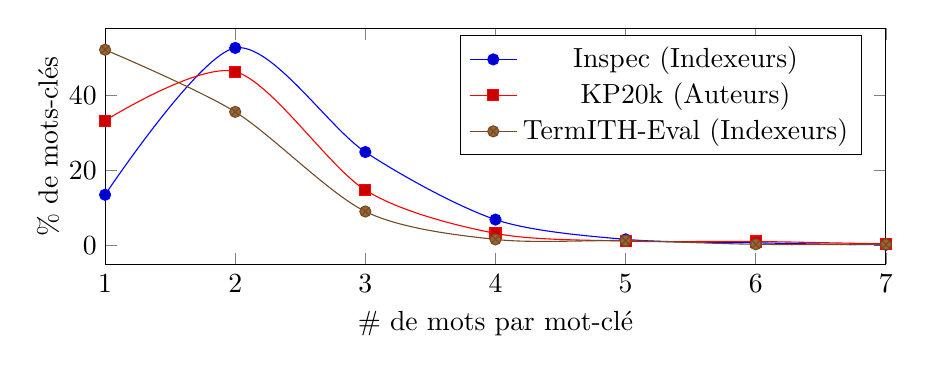
\begin{tikzpicture}
\begin{axis}[
    smooth,
    scale only axis,
    width=\textwidth-0.1cm-60,
    height=3cm,
    yticklabel style={inner sep=0pt, align=right, xshift=-0.1cm},
    xmin=1, xmax=7,xtick={1,2,3,4,5,6,7},
    xlabel={\# de mots par mot-clé},
    ylabel={\% de mots-clés},
    legend pos=north east]

\addlegendentry{Inspec (Indexeurs)}
\addplot coordinates {
    (1, 13.4337472)(2, 52.59515571)(3, 24.83207816)(4, 6.81864441)(5, 1.54691634)(6, 0.63097904)(7, 0.10177081)(9, 0.04070832)};
%\addlegendentry{KDD}
%\addplot coordinates {
%    (1, 25.47688328)(2, 56.22373101)(3, 14.03168445)(4, 3.55641772)(5, 0.54962819)(6, 0.06466214)(7, 0.03233107)(8, 0.06466214)};
\addlegendentry{KP20k (Auteurs)}
\addplot coordinates {
    (1, 33.21207643)(2, 46.26992924)(3, 14.69292636)(4, 3.13468042)(5, 1.08752285)(6, 0.97289719)(7, 0.35713947)(8, 0.11273103)(9, 0.0435767)(10, 0.03126155)(11, 0.01799907)(12, 0.01420979)(13, 0.0094732)(14, 0.0047366)(15, 0.01136783)(16, 0.00284196)(17, 0.00284196)(18, 0.00284196)(19, 0.00378928)(20, 0.00378928)(21, 0.00094732)(23, 0.00189464)(24, 0.00094732)(25, 0.00094732)(27, 0.00094732)(28, 0.00284196)(33, 0.00094732)(105, 0.00094732)};
\addlegendentry{TermITH-Eval (Indexeurs)}
\addplot coordinates {
    (1, 52.11118184)(2, 35.53999576)(3, 8.97517505)(4, 1.52768937)(5, 1.20942075)(6, 0.23339699)(7, 0.19096117)(8, 0.04243582)(9, 0.02121791)(10, 0.06365372)(12, 0.02121791)(14, 0.02121791)(15, 0.02121791)(16, 0.02121791)};
\end{axis}
\end{tikzpicture}


    \caption{Nombre de constituants par mot-clé dans les ensembles de test de différents jeux de données.}
    \label{fig:tok_per_kw_abstract}
\end{figure}

Pour aider les auteurs à choisir les mots-clés de leurs articles, \citet{gbur_key_1995} donnent des recommandations pour l'anglais.
Par exemple, ils recommandent de ne pas répéter les mots-clés des titres, de ne pas choisir de mots-clés trop communs (\say{regression} dans le domaine des statistiques) et de choisir des syntagmes nominaux simples et spécifiques qui évitent les composés syntagmatiques avec groupe prépositionnel (\say{reliability} plutôt que \say{theory of reliability}) etc.


%TermITH-Eval:
%-9; benzènesulfonique acide(méthyl-4) [méthyl-«5p» isoxazolyl-«3p»] amide
%-12; samovar (système d'analyse et de modélisation des validations et des automobiles renault)
%-6; grammaire syntagmatique menée par la tête
%KP20k:
%-16; low n/d n / d ratio n/d n / d n/d n / d n / d
%-9; decision support system for construction and retrofit projects (dss-crp)
%-11; large-scale nonlinear least-squares problems subject to dynamical system constraints
%Inspec:
%-9; iterative regularized least-mean mixed-norm image restoration
%-7; automatic teller machine computer-based voting system


\subsection{Mots-clés présents et mots-clés absents}
\label{sub:mots-cles-present-et-absent}

La notion d'absence d'un mot-clé a été introduite et formalisée par~\citet{meng_deep_2017} dans les termes suivants:
\say{[...] nous dénotons les mots-clés qui ne correspondent à aucune sous-séquence continue du texte source comme des mots-clés absents, et ceux qui correspondent à une partie du texte comme des mots-clés présents}.\footnote{\say{\foreign{[...] we denote phrases that do not match any contiguous subsequence of source text as absent keyphrases, and the ones that fully match a part of the text as present keyphrases.}}}
Cette définition est implémentée en cherchant si la séquence de mots du mot-clé apparaît dans le même ordre que dans la séquence de mots du texte source.\footnote{\href{https://github.com/memray/seq2seq-keyphrase/blob/9145c63ebdc4c3bc431f8091dc52547a46804012/keyphrase/keyphrase\_utils.py\#L96}{\texttt{github.com/memray/seq2seq-keyphrase/keyphrase/keyphrase\_utils.py\#L96}}}
Ce découpage permet de différencier les mots-clés pouvant être extraits du document (mots-clés présents) de ceux devant être générés (mots-clés absents).
Cette différenciation est généralement utilisée pour filtrer la référence et pour évaluer une méthode sur sa seule capacité à extraire ou à générer des mots-clés.
Les méthodes extractives ont historiquement été évaluées à l'aide de la référence entière. Aujourd'hui il est commun d'évaluer séparément les mots-clés présents et les mots-clés absents~\cite{meng_deep_2017, sun_divgraphpointer_2019}.
%
%En effet, les méthodes de génération de mots-clés sont bien meilleures pour produire des mots-clés présents que pour produire des mots-clés absents.
%De plus, les méthodes extractives neuronales sont évaluées sur les seuls mots-clés présents.


\section{Méthodes en chaîne de traitement}\label{sec:methode-en-chaine-de-traitement}
Dans cette section, nous présentons les méthodes d'extraction automatique de mots-clés en chaîne de traitement.
Ces méthodes sont dites en \say{chaîne de traitement} car elles s'exécutent en trois étapes:
\begin{enumerate}
    \item l'identification d'unités textuelles que l'on va considérer comme candidates à être des mots-clés;
    \item la pondération de ces mots-clés candidats, à l'aide de différentes méthodes: statistiques, de classification, utilisant des graphes, etc.~;
    \item la sélection d'un sous-ensemble de candidats qui représente le document.
\end{enumerate}
La figure~\ref{fig:chaine_traitement} illustre le déroulement en trois étapes des méthodes en chaîne de traitement.


\begin{figure}[htbp]
    \centering

    \begin{tikzpicture}[scale=1.5, transform shape]
    \tikzstyle{label}=[text width=3 cm, align=center, scale=.75]
    
    \pic[local bounding box=doc1] {doc={scale 2}};
    \node[above=.25 of doc1, label] (label1) {Pré-traitements linguistiques};

    \pic[local bounding box=doc2, right=1.5 of doc1] {dockw={scale 2}};
    \node[above=.25 of doc2, label] (label2) {Identification des candidats};

    \pic[local bounding box=weighted, right=1.5 of doc2] {weighted={scale 1}};
    \node[above=.35 of weighted, inner xsep=-.125cm, label] (label3) {Pondération des candidats};

    \pic[local bounding box=kws, right=1.5 of weighted] {kws={scale 1}};
    \node[above=.45 of kws, inner xsep=-.1cm,label] (label4) {Sélection du sous-ensemble};
    
    \node[below=.1 of doc2, inner xsep=-.125cm, label, scale=.75] (step1) {\'Etape 1};
    \node[inner xsep=-.125cm, label, scale=.75] (step2) at (step1 -| weighted) {\'Etape 2};
    \node[inner xsep=-.125cm, label, scale=.75] (step3) at (step1 -| kws){\'Etape 3};

    \draw[->, thick] (doc1) -- (doc2);
    \draw[->, thick] (doc2) -- (weighted);
    \draw[->, thick] (weighted) -- (kws);

    \end{tikzpicture}
    
    \caption{Étapes principales des méthodes d'extraction de mots-clés en chaîne de traitement.}
    \label{fig:chaine_traitement}
\end{figure}



\subsection{Identification des mots-clés candidats}\label{selection-des-mots-cles-candidats}

% le filtrage de la redondance et autre? peut se faire soit à cette étape soit quand on choisis le sou-ensemble
L'identification des mots-clés candidats est la première étape de l'extraction de mots-clés. Elle consiste à identifier certaines unités textuelles du document qui peuvent être des mots-clés.
Cette identification met en \oe{}uvre des heuristiques exploitant certaines caractéristiques des mots-clés (fréquence, position, patron morphosyntaxique, \ldots).
Le choix de la méthode de sélection des mots-clés candidats influe grandement sur la tâche d'extraction car elle pose une hypothèse forte sur les propriétés que doivent respecter les mots-clés.
Sélectionner un grand nombre de candidats complexifie l'étape suivante de pondération. En sélectionner trop peu risque de limiter les performances de l'extraction de mots-clés en occultant certains mots-clés pertinents.
%En effet si aucun mots-clés de référence n'est sélectionné à cette étape, la méthode ne pourra les pondérer et aura un score de 0.
% entre nombre de cand et rappel max, bruit
% enlever les redondants 
Cette étape doit donc trouver un compromis entre minimiser le bruit (le nombre de candidats non pertinents) et maximiser le rappel (le nombre de candidats pertinents).


Deux  méthodes principales sont employées pour la sélection de mots-clés~: les n-grammes et les patrons morphosyntaxiques.
Les n-grammes (séquences continues de $n$ mots) sélectionnés sont  généralement des unigrammes, bigrammes et trigrammes~\cite{witten_kea:_1999,campos_yake_2020}. Cette méthode produit un nombre conséquent de mots-clés candidats mais elle garantie une couverture de l'ensemble du document.
Les n-grammes candidats sont ensuite filtrés pour éliminer les séquences peu susceptibles d'être des mots-clés, comme celles qui commencent et finissent par des catégories grammaticales fonctionnelles ou encore celles qui ne contiennent ni nom ni adjectif.

% (N|A)+
Les méthodes les plus populaires sélectionnent des séquences d'étiquettes morphosyntaxiques à l'aide de patrons morphosyntaxiques. 
Nous avons vu dans la section~\ref{sub:nature_linguistique} que les mots-clés sont en grande majorité composés de noms et d'adjectifs.
Le patron générique le plus populaire est \texttt{/(NOUN|ADJ)+/}~\cite[\textit{inter alia}]{mihalcea_textrank:_2004,wan_collabrank:_2008,bougouin_topicrank:_2013}. %, un patron plus précis que l'on retrouve dans la figure~\ref{fig:patron_syntaxique_kp20k} est \texttt{/ADJ? NOUN+/}.
Construire des patrons morphosyntaxiques plus précis, décrivant des mots-clés, requiert soit l'expertise linguistique de spécialistes de la langue, soit l'acquisition automatique de patrons à partir d'un ensemble d'apprentissage annoté en mots-clés.
Dans cette direction, \citet{hulth_improved_2003} considère comme patrons acceptables tous les patrons apparaissant au moins 10 fois dans les mots-clés des documents d'entraînement.
Les outils d'étiquetage morphosyntaxique sont aujourd'hui des outils de traitement linguistique de base pour de nombreuses langues à l'exception de certaines langues peu dotées.
En terme de performances, l'étiqueteur morphosyntaxique de l'outil \texttt{spacy}\footnote{\url{https://spacy.io/models}} atteint une précision de \npercent{97} pour l'anglais et \npercent{93} pour le français.
Ces bonnes performances globales cachent néanmoins des problèmes récurrents :
en anglais, un problème d'étiquetage des extensions du nom de tête des composés anglais par exemple dans \say{\foreign{ant colony optimization}}, \foreign{ant} est catégorisé comme adjectif au lieu de nom ;
en français, la confusion de noms en verbes dès que la forme du nom est aussi une forme flexionnelle acceptable du verbe, par exemple le nom \say{défigement} fini par \say{ent} et est catégorisé comme verbe.
Pour le français, par exemple, les mots-clés peuvent contenir des prépositions comme \say{langue \textit{de} spécialité}; le patron \texttt{(NOUN|ADJ)+} ne permet pas la sélection de ces composés nominaux pourtant très fréquents~\cite{daille_term_2017}.
% neural network / réseau de neurone

%Il est aussi possible d'identifier les candidats en utilisant un vocabulaire contrôlé provenant d'un thésaurus ou autre référentiel. Cette méthode assure des candidats de qualité et cohérents entre les documents mais ne permet pas d'avoir une couverture exhaustive~\cite{willis_2013_bs}.

La figure~\ref{fig:ex_selection} donne un exemple de candidats sélectionnés par la méthode n-grammes et selon le patron \texttt{/(NOUN|ADJ)+/}. Le nombre de candidats identifiés en conservant les n-grammes de 1 à 3 (12 candidats) est très supérieur à ceux identifiés par le patron \texttt{/(NOUN|ADJ)+/} (2 candidats).
La plupart des candidats identifiés par la méthode n-gramme n'apporte que peu d'informations quant aux sujets du document.

\begin{figure}[!htbp]
    \centering
    \begin{tabular}{ll}
        \multirow{2}{*}{1-grammes} & indexation ; libre ; ensemble ; unités ;\\
         & descriptives ; utilisés ; connu ; priori\\
         \cmidrule(lr){1-2}
        2-grammes & indexation libre ; unités descriptives\\
         \cmidrule(lr){1-2}
        3-grammes & ensemble des unités ; connu a priori\\
         \cmidrule(lr){1-2}
        Patron \texttt{(N|A)+} & indexation libre ; unités descriptives \\
    \end{tabular}
    \caption{Mots-clés candidats identifiés par la méthode n-grammes et selon le patron \texttt{(NOUN|ADJ)+} dans la phrase \say{\textit{Dans l'indexation libre, l'ensemble des unités descriptives qui peut être utilisé n’est pas connu a priori.}} provenant de \citet{neveol_automatisation_2005}.}
    \label{fig:ex_selection}
\end{figure}



\subsection{Pondération des mots-clés candidats}\label{ponderation}
L'étape de pondération des mots-clés candidats consiste à leur assigner un score évaluant leur potentialité à être un mot-clé.
Nous présentons les méthodes de l'état de l'art en les regroupant par catégories: les méthodes statistiques qui utilisent des statistiques descriptives, les méthodes utilisant des graphes pour représenter les documents, les méthodes de classification supervisées et d'autres méthodes ne rentrant pas dans ces catégories.

\subsubsection{Méthodes statistiques}\label{statistique}

La méthode statistique la plus utilisée est le \tfidf{}~\cite{jones_statistical_1972}.
C'est une méthode de référence très populaire dans la plupart des tâches de traitement automatique de la langue. Le \tfidf{} est un schéma de pondération qui exploite la fréquence des mots dans une collection de documents.
Sa formule est décrite dans l'équation~\ref{eq:tfidf} avec $N$ le nombre de documents de la collection, $\textsc{Df}(w)$ le nombre de documents comportant le mot $w$, $\textsc{Tf}_d(w)$ le nombre d'occurrences du mot $w$ dans le document $d$.
L'idée étant que la fréquence élevée d'un mot ou sa spécificité à un document sont des indicateurs d'importance de ce mot. 

\begin{align}
    \tfidf(d, w) = & \textsc{Tf}_d(w) * log\left( \frac{N}{\textsc{Df}(w)} \right) \label{eq:tfidf}
\end{align}

%Avec $N$ le nombre de documents de la collection, $\textsc{Df}(w)$ le nombre de documents comportant le mot $w$, $\textsc{Tf}_d(w)$ le nombre d'occurrences du mot $w$ dans le document $d$.%, $|d|$ le nombre de mots du document $d$ et $avgdl$ le nombre moyen de mots par documents dans la collection. $b$ et $k_1$ sont des constantes permettant de modifier l'importance de la longueur du document ($b$ est généralement fixé à \num{0.75}).

%L'idée étant qu'un mot ayant une fréquence élevée ou qu'il soit spécifique à un document sont des indicateurs d'importance du mot. 
%L'intérêt de \bm{} par rapport a \tfidf{} est d'augmenter l'importance d'un mot dans un document si le document est plus court.

Outre la fréquence, la position d'un candidat dans le document est un indicateur fort de sa propension à être un mot-clé. La position est utilisée dans plusieurs méthodes~\cite[\textit{inter alia}]{witten_kea:_1999,goh_keyphrase_2007,campos_yake_2020} que nous décrivons ensuite.
C'est en effet au début d'un article scientifique, dans son titre et son résumé, que l'on va mentionner les concepts décrits dans l'article.
Dans la tâche de résumé automatique, la méthode de base, à laquelle se comparer, utilise les premières phrases du document qui sont utilisées comme résumé~\cite{brandow_automatic_1995}.
La méthode \say{FirstPhrases}~\cite{gallina_large-scale_2020} s'inspire de cette méthode et ordonne les candidats selon leur position dans le document.

\iffalse
\begin{align}
    \text{score}(d, w) = & \frac{pos(w)}{|d|}) \label{eq:firstphrases}
\end{align}
\fi

La méthode YAKE!~\cite{campos_yake_2020} est une méthode qui calcule le score des candidats à l'aide de plusieurs descripteurs statistiques.
L'intérêt de ces descripteurs est qu'ils sont indépendants de la langue et -- à l'inverse de \tfidf{} -- ne nécessitent pas de collection de documents.
En plus de la fréquence et de la position, la casse et les coocurrences sont aussi utilisées.

%Tous ces descripteurs sont ici utilisé de manière non supervisés mais peuvent être inclus dans des méthodes supervisés.


\subsubsection{Méthodes de classification}\label{classification}

L'extraction de mots-clés peut être reformulée comme une tâche de classification binaire. Chaque candidat est classé comme mot-clé ou non mot-clé. La confiance du classifieur dans sa prédiction peut être utilisée pour donner un score aux candidats et donc pour les classer.
%Ces méthodes ont été peu développées à cause de la faible disponibilités d'ensemble d'apprentissage dans les jeux de données distribués, mais les quelques 


La méthode historique Kea~\cite{witten_kea:_1999} combine seulement deux descripteurs pour classifier les mots-clés candidats: le \tfidf{} et la position de la première occurrence.
Cette méthode bien que simple est aujourd'hui toujours compétitive, elle exploite la fréquence et la position qui sont deux caractéristiques fortement liées à l'importance d'un mot.

Certaines méthodes se concentrent sur l'extraction de mots-clés dans les articles scientifiques et peuvent ainsi tirer parti de leur structure.
Dans leurs travaux \citet{goh_keyphrase_2007} remarquent que les mots-clés n'apparaissent pas de manière équiprobable dans toutes les sections des articles scientifiques.
Pour prendre en compte cette information, un classifieur détecte l'apparition d'un mot-clé candidat dans 14 types de sections avec une précision de \npercent{92}.
Parmi ces 14 types de sections se trouvent: le résumé, l'introduction, la conclusion, les travaux connexes, les références, etc.
Cette information est ensuite utilisée comme trait supplémentaire pour classifier les mots-clés candidats.
%En plus du \tfidf{}, de la position) et de descripteurs morphologiques (le patron morphosyntaxique, le suffixe et si le mot est un acronyme), un vecteur indiquant les sections du document dans lesquelles apparaît le candidat est ajouté pour l'entraînement d'un classifieur NaiveBayes.

%Une des premières méthode à utiliser un réseau de neurones est \cite{sarkar_new_2010}. Les descripteurs utilisés sont la fréquence, la position et la longueur du candidats.

\subsubsection{Méthodes fondées sur les graphes}\label{graphe}

Les méthodes fondées sur les graphes sont très populaires pour l'extraction de mots-clés. Les graphes permettent de calculer des mesures de centralité des n\oe{}uds qui dénotent leur importance.
%Les graphes peuvent être utilisés pour modéliser les unités textuelles au sein d'un document ou d'une collection de documents.
Dans le cadre de l'extraction de mots-clés, le graphe $G=(V, E)$ est composé de noeuds $V$, qui représentent les mots d'un document, et d'arêtes $E$, qui représentent les relations de cooccurrence entre les mots selon une fenêtre glissante de $n$ mots.

%Les noeuds sont pondérés grâce à un algorithme de marche aléatoire qui calcule leur popularité, en fonction de la popularité des noeuds voisins.

La méthode pionnière utilisant des graphes est TextRank~\cite{mihalcea_textrank:_2004}.
Cette méthode applique l'algorithme PageRank~\cite{page_pagerank_1999} pour pondérer les noeuds et donc les mots du document.
L'idée de cet algorithme est qu'un mot est important s'il cooccurre avec un grand nombre de mots, et si les mots avec lesquels il cooccurre sont eux aussi importants.
Ensuite, les candidats sont pondérés en sommant les scores des mots qui les composent.
Cette méthode, bien que précurseure, obtient généralement des performances assez basses. D'autres méthodes ont été présentées pour l'améliorer.

%L'algorithme PageRank est un algorithme de marche aléatoire dans un graphe qui calcule le score des noeuds de manière itérative selon l'équation~\ref{eq:textrank}.
%Cet algorithme a été créé pour le référencement des pages du web et modélise le parcours de navigation d'un·e internaute.
%Les arêtes représentent les liens entre les pages web, la partie droite de l'équation modélise la probabilité d'arriver à la page $V_i$ à partir de la page $V_j$ sachant son importance $S(V_j)$. La partie gauche $d$ (\emph{damping factor}) -- fixé a 0.85~\cite{brin_anatomy_1998} -- représente la probabilité de changer de page sans cliquer sur un lien.
%
%Dans l'équation~\ref{eq:textrank} $S$ est un vecteur de longueur $|V|$ qui représente le poids de chacun des noeuds. $\textsc{In}(V_i)$ et $\textsc{Out}(V_i)$ représentent respectivement les noeuds possédant des arcs entrants ou sortant vers $V_i$. \todo{Je rajouterai un exemple de simulation de cet algo.}

%\begin{align}
%S(V_i) = & (1 - d) + d * \sum_{j\in\textsc{In}(V_i)} \frac{W_{ji}}{\sum_{k\in\textsc{Out}(V_j)} W_{jk}} S(V_j) \label{eq:textrank}
%\end{align}

Les méthodes CollabRank~\cite{wan_collabrank:_2008}\footnote{Parfois nommée ExpandRank.} et CiteTextRank~\cite{gollapalli_extracting_2014} s'inspirent de TextRank et améliorent la représentation sous forme de graphe grâce à des données supplémentaires.
CollabRank crée le graphe à partir du document et de documents proches identifiés grâce à un algorithme de regroupement (\textit{clustering}), tandis que CiteTextRank traite les articles scientifiques et ajoute au graphe les contextes de citations de l'article.
CiteTextRank semble obtenir de meilleures performances que CollabRank mais nécessite d'avoir accès à des articles scientifiques ainsi qu'à leurs contextes de citation. Malheureusement, ces informations sont peu disponibles et difficilement accessibles.

%\todo{Ajouter un graphe avec des mots et des poids pour les noeuds ?}
% Il faudrait prendre un doc, et avec pke afficher le poids de chacun des mots, ensuite pour l'afficher avec graphviz
% La figure~\ref{aaa} présente le graphe d'un document après exécution de l'algorithme TextRank. Les mots a, b et c sont les plus centraux.

Les méthodes TopicalPageRank~\cite{liu_automatic_2010}, TopicRank~\cite{bougouin_topicrank:_2013} et son amélioration MultipartiteRank~\cite{boudin_unsupervised_2018} améliorent TextRank en regroupant par sujets les mots du document ou les candidats.
TopicalPageRank utilise le LDA pour calculer les sujets auxquels appartiennent les mots. Le LDA~\cite{blei_latent_2003} (\foreign{Latent Dirichlet Allocation}) est une technique de modélisation en sujets qui s'inscrit dans les techniques de réduction de dimensionalité. Le LDA est un modèle statistique génératif qui permet de représenter un document en une mixture de sujets, à leur tour représentés par une mixture de mots.
L'algorithme PageRank est biaisé pour prendre en compte l'apport des mots dans chacun des sujets.
Les méthodes TopicRank et MultipartiteRank quand à elles, regroupent les mots-clés candidats sur la base du nombre de mots communs. Cette technique est plus simple que LDA mais ne requiert pas d'entraînement.
Ces deux méthodes, contrairement à TextRank et à la majorité des autres méthodes, modélisent les candidats plutôt que les mots et forment un graphe complet en pondérant les arêtes par la distance entre les candidats dans le document.


Parmi les méthodes proposées, certaines modifient TextRank en biaisant l'algorithme PageRank pour prendre en compte une caractéristique importante des mots-clés. Par exemple PositionRank~\cite{florescu_positionrank:_2017} biaise PageRank en fonction des positions des mots dans le document.
Ce seul changement apporte un gain de performance important par rapport à TextRank qui montre l'intérêt de cette caractéristique pour l'identification de mots-clés.

Dans la grande majorité des méthodes présentées, la construction du graphe et la pondération des arêtes sont basée sur les relations de cooccurrences. Pour tenter de capturer les relations sémantiques entre les mots,  \citet{mothe_automatic_2018} étudie l'utilisation de la similarité sémantique pour pondérer les arêtes du graphe à l'aide de plongements de mots statiques.
Leurs expériences montrent que l'utilisation des plongements de mots seul ou leur combinaison avec la coocurence n'apportent pas de gain de performances significatif.
%\begin{align}
%S(V_i) = & \sum_{j\in\textsc{In}(V_i)} \frac{W_{ji}}{\sum_{k\in\textsc{Out}(V_j)} W_{jk}} S(V_j) * d + P(V_i) * (1 - d) \label{eq:positionrank} \\[.5em]
%P(V_i) = & \frac{\Tilde{P}(V_i)}{\sum_{j\in \Tilde{P}} \Tilde{P}(V_j)}
%\end{align}

%Où $\Tilde{P}$ est un vecteur de dimension $|V|$ qui représente la position du mot. $\Tilde{P}(V_i)$ est la somme de l'inverse des positions de ses occurrences.
%Si un mot apparaît en 2\textsuperscript{d}, 5\textsuperscript{e} et 32\textsuperscript{e} position dans le document, alors $\Tilde{P}(V_i) = \frac{1}{2} + \frac{1}{5} + \frac{1}{32}$. $P$ est la version normalisée de $\Tilde{P}$.

\subsubsection{Autres méthodes}

Une des premières méthodes à exploiter les représentations denses de mots pour l'extraction de mots-clés non supervisée est  EmbedRank~\cite{bennani-smires_simple_2018}.
Cette méthode pondère les mots-clés candidats en fonction de leur distance sémantique au document.
Pour calculer cette distance sémantique, le document et les mots-clés candidats sont d'abord représentés sous forme vectorielle grâce à une technique de plongements de phrases ~\cite{pagliardini_unsupervised_2018}. Enfin, le poids est calculé par la distance cosinus entre le vecteur du document et les vecteurs des candidats.


La méthode TopicCoRank~\cite{bougouin_indexation_2015} est une méthode fondée sur les graphes qui utilise l'ensemble des mots-clés de référence pour pouvoir prédire des mots-clés n'apparaissant pas dans le document.
Pour cela, l'ensemble des mots-clés de référence d'un jeu de données sont représentés dans un \say{graphe du domaine} dans lequel deux mots-clés sont connectés s'il apparaissent dans les mêmes ensembles de référence.
Ce graphe du domaine est connecté au graphe du document\footnote{Construit de la même manière que pour TopicRank.} par les mots-clés communs aux deux graphes.
De manière similaire aux autres méthodes fondées sur les graphes, l'algorithme PageRank pondère les n\oe{}uds (dont ceux du graphe du domaine).
La pondération du graphe du domaine permet donc à cette méthode de retourner des mots-clés absents du document, c'est une des rares méthodes en chaîne de traitement à permettre cela.

%\subsubsection{Assignation de mots-clés}\label{autre}
% plus proche de classification
%La tâche d'assigner des mots-clés à un document peut être vue comme une tâche de classification multi-étiquettes, où les étiquettes sont les mots-clés.
%Cette formulation de la tâche implique qu'il existe un nombre fini de mots-clés, par exemple dans le domaine médical avec le thésaurus MeSH.
%La tâche partagée proposée par BioASQ 2013~\cite{partalas_results_2013} est d'associer les mots-clés du MeSH à des articles scientifiques médicaux.
%Certaines méthodes proposées entraînent des classifieurs à calculer une probabilité pour chaque mot-clé d'être associé à un document.

%\cite{tomokiyo_language_2003} Language model difference
%\cite{liu_automatic_2011} modèle de généartion précurseur

\subsection{Sélection du sous-ensemble de mots-clés}\label{choisir-le-sous-ensemble}

% pas ou peu exploré
Une fois les mots-clés candidats pondérés, il est nécessaire de sélectionner un sous-ensemble de candidats que l'on va considérer comme mots-clés.
L'approche la plus simple consiste à sélectionner les $n$ candidats ayant les meilleurs scores.
Le choix du $n$ peut être lié entre autre à la longueur du document ou l'utilisation qui sera faite des mots-clés. % peu de travaux ont travaillé
Ce sont, le plus souvent, les 5 ou 10 premiers mots-clés qui sont choisis, ces chiffres correspondent au nombre moyen de mots-clés annotés par les auteurs et les indexeurs professionnels (cf. section~\ref{sec:framework_datasets}).
La problématique du choix du nombre de mots-clés à associer à un document n'est pas résolue.
Certaines méthodes proposent de choisir ce nombre en fonction de la longueur du document~\cite{mihalcea_textrank:_2004}, ou d'entraîner un modèle à produire le bon nombre de mot-clés~\cite[\textit{inter alia}]{yuan_generating_2018, chen_exclusive_2020}.

Lors du choix des mots-clés une étape de filtrage peut être exécutée pour supprimer les mots-clés redondants~\cite{hasan_automatic_2014}.
Les mots-clés qui sont contenu dans un mot-clé mieux classé sont généralement redondants. Par exemple si le mot-clé \say{indexation libre} est mieux classé que \say{indexation}, ce dernier sera considéré comme redondant.

\section{Conclusion}

Nous avons présenté dans ce chapitre les concepts importants posant le contexte de cette thèse ainsi que les méthodes de production automatique de mots-clés en chaîne de traitement.

L'annotation de mots-clés, pour être effectuée manuellement, requiert de nombreuses ressources en terme d'indexeurs professionnels, de temps et de moyens financiers.
C'est pourquoi la production automatique de ces mots-clés est un enjeu important pour les bibliothèques numériques scientifiques.

Les méthodes précurseures de cette tâche sont dites \say{en chaîne de traitement} car elles consistent en trois étapes: l'identification de mots-clés candidats, leur pondération puis la sélection d'un ensemble de mots-clés.
Chacune de ces étapes est cruciale pour la suivante, si les mots-clés candidats sélectionnés sont peu qualitatifs alors les mots-clés en sortie le seront aussi.
La communauté scientifique propose de nombreuses méthodes qui exploitent des caractéristiques telles que la fréquence, la position et la centralité des mots pour extraire les mots-clés des documents.
Malgré les avancées de ces méthodes, les performances sont limités par la propagation des erreurs, inhérente aux méthodes en chaîne de traitement, ainsi que le choix des traits utilisé, issus de connaissance expertes.
C'est pourquoi des méthodes de bout-en-bout, que nous décrivons dans le chapitre~\ref{chap:kw_production}, ont été développées.
